\chapter{ファイルシステムの概念}
\label{fileSystemConcepts}
ファイルシステムは二次記憶装置(ストレージ)を管理・抽象化・仮想化し,
使いやすいファイルをユーザに提供する.
ファイルは,名前が付けられた一次元のバイト列(\emph{バイトストリーム})である.
オペレーティングシステムはバイト列の使い方を規定しない.
名前で一つのファイルを指定し,
その中のバイト位置でデータを指定することができる.

%現代のOSではファイルは単なるバイト列であるが,
%過去のOSにはファイルが構造を持つものもあった.
%これらのファイルシステムでは現代のデータベースのように
%キーでファイル内を検索したり,
%キーの順になるようにデータをファイルの途中に挿入したりすることができた.
%(ISAMの話を入れると良さそうだが自信なし)

%============================================================================
\section{ファイルの名前付け}
ファイルは木構造の\emph{ディレクトリシステム}に格納される\footnote{
  現代のオペレーティングシステムでは,ほとんどの場合,そうである.}.
\figref{dirTree}に木構造の例を示す.
ディレクトリ\footnote{WindowsやmacOSではフォルダとも呼ぶ.}は,
他のディレクトリやファイルの名前とファイル本体へのポインタ\footnote{
  多くの場合はファイル本体に付けられたユニークな番号である.
}の組を記録する特殊なファイルである.
木構造の中から一つのファイルを特定するために,
階層構造を持った名前(\emph{パス})を用いる.
パスには絶対パスと相対パスの二種類がある.

\begin{myfig}{btp}{木構造のディレクトリシステム}{dirTree}
  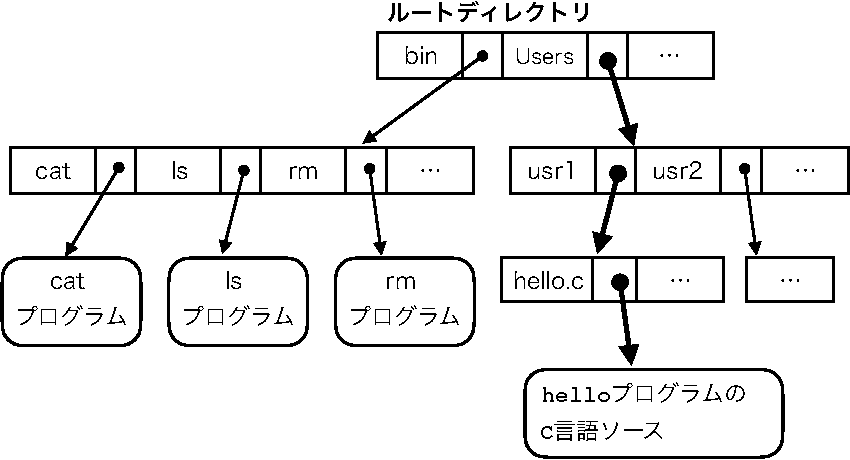
\includegraphics[scale=.8]{Fig/dirTree-crop.pdf}
\end{myfig}

\begin{itemize}
\item \emph{絶対パス} \\
  木構造の根にあたる\emph{ルートディレクトリ}を起点に
  目的のファイルへ辿り着く道順を書き表したものを絶対パスと呼ぶ.
  例えば,\figref{dirTree}の「helloプログラムのC言語ソース」
  ファイルの絶対パスは,\|/Users/usr1/hello.c|である.
  絶対パスは「\|/|」から書き始める.

\item \emph{相対パス} \\
  プロセスは,現在の操作対象になる一つの
  \emph{ワーキングディレクトリ(カレントディレクトリ)}を持つ.
  相対パスは,ワーキングディレクトリを起点に
  目的のファイルへ辿り着く道順を書き表したもである.
  例えば,\figref{dirTree}の\|/Users|ディレクトリが
  ワーキングディレクトリの場合,
  「helloプログラムのC言語ソース」ファイルは相対パスは\|usr1/hello.c|になる.
  相対パスは「\|/|」\emph{以外}から書き始める.
\end{itemize}

%============================================================================
\section{ファイルの別名}
ファイルを別名で参照できると便利なことがある.
例えば,その日の作業記録ファイルを,毎日,作成するシステムがあるとする.
このシステムではファイル名の一部に年月日を埋込むことで区別し,
過去3日分を消さずに残すものとする.
しかし,最新のファイルはいつも同じ名前でアクセスできると便利だ.
そこで、最新のファイルに綴りが変化しない別名を付ける.
次のような状態である.

\begin{center}
  \begin{tabular}{l l}
    %\multicolumn{1ファイル名
    \texttt{2017\_06\_30.log}   & 2017年6月30日のファイル \\
    \texttt{2017\_07\_01.log}   & 2017年7月1日のファイル  \\
    \texttt{2017\_07\_02.log}   & 2017年7月2日のファイル  \\
    \texttt{today.log}          & 現時点では2017年7月2日のファイルの別名
  \end{tabular}
\end{center}

このような別名の仕組みとして大きく3つの方式が考えられる.

\begin{itemize}
\item \emph{ハードリンク} \\
  主にUNIXで使用される方式である\footnote{macOSやWindowsでも使用できる.}.
  ファイルシステムの仕組みとしてOSカーネルに組込む.
  \figref{dirTree}で,同一のファイル本体を指すポインタが
  複数のディレクトリ・エントリに存在する状態である\footnote{
    ファイル本体が複数の箇所から指されるので,
    ディレクトリシステムが木構造ではなく非循環グラフになってしまう.}.
  ファイル本体には何ヶ所から指されているか管理するリンクカウントを設置し,
  リンクが削除されカウントがゼロになった時点でファイル本体を削除する.

  原理的にはディレクトリファイルをリンクすることも可能であるが,
  リンクのループを作ることが可能になってしまう\footnote{
    ディレクトリシステムが一般グラフになる.}のでUNIXでは許されていない.
  ループを許可すると,
  ルートディレクトリから分離した離れ小島状態の部分木が出来た時,
  リンクカウントが永遠にゼロにならない問題が生じる.
  ループの検出はコストが高い処理なので最初からディレクトリのリンクを禁止する.

\item \emph{シンボリックリンク} \\
  主にUNIXで使用される方式である\footnote{macOSやWindowsでも使用できる.}.
  ファイルシステムの仕組みとしてOSカーネルに組込む.
  シンボリックリンクは他のファイルのパスをデータとして
  格納した特別なファイルだと考えられる.
  シンボリックリンクファイルはOSカーネルが特別な扱いをする.

  シンボリックリンクは,使用時に格納されたパスを評価し直すので,
  オリジナルファイルの名前を変更するとリンク切れ状態になる.
  同じ名前で新たに別のファイルが作られると,それへのリンクに変わる.
  リンク先が存在しないシンボリックリンクを作ることもできる.
  シンボリックリンクの特徴は,
  リンクが切れて新しいファイルに勝手に接続されることである.

\item \emph{ファイルシステムの外で実装されるリンク} \\
  WindowsのショートカットやmacOSのエイリアスがこれにあたる.
  ハードリンクやシンボリックリンクはOSカーネル内で処理され,
  リンクの存在がアプリケーションからは透過(透明)なので,
  とてもスマートな仕組みに見える.
  しかし,現代のオペレーティングシステム(例えばmacOS)では,
  オペレーティングシステムはローカルハードディスクの
  HFS+ファイルシステムにインストールし,
  ユーザのホームディレクトリはネットワークドライブに格納され
  SMBプロトコルでアクセスし,
  デジカメのデータをマイクロSDから読込む時はFATファイルシステムを使用する.
  使用するファイルシステムが何種類もあるので,
  統一的に使用できるリンクの仕組みが保証されない\footnote{
    例えばFATファイルシステムにはハードリンクや
    シンボリックリンクの仕組みはない.}.
  そこで,アプリケーションやライブラリ(もしかしたらOSカーネル内)等,
  ファイルシステムの外にリンクの代替となる仕組みを準備していることがある.

  \begin{itemize}
  \item \emph{HFS+上のmacOSのエイリアスの例} \\
    HFS+ファイルシステム上でエイリアスは拡張属性(\ref{fileAttribute}参照)を
    持った普通のファイルとして格納される.
    ファイルシステムが提供する汎用的な機構である
    拡張属性をエイリアスの実現に利用しているだけで,
    エイリアス専用の機能をファイルシステムが持つ訳ではない.
    リスト\ref{aliasOnHFS}にHFS+ファイルシステム上のエイリアスの例を示す.
    3,4行からファイル「\|a.txtのエイリアス|」が
    32バイトの拡張属性\|com.apple.FinderInfo|を持つことが分かる.

    \lstinputlisting[caption=HFP+ファイルシステム上のmacOSのエイリアス,
      numbers=left,label=aliasOnHFS,float=btp]{Lst/aliasOnHFS.txt}

  \item \emph{FAT上のmacOSのエイリアスの例} \\
    FATファイルシステム上ではエイリアス本体と
    拡張属性を格納する二つの通常ファイルとして作成される.
    ファイルの内容を解釈する時点で拡張属性を実現している.
    リスト\ref{aliasOnFAT}にFATファイルシステム上のエイリアスの例を示す.
    4,5行からファイル「\|a.txtのエイリアス|」が
    32バイトの拡張属性\|com.apple.FinderInfo|を持つことが分かる.
    リスト\ref{aliasOnFAT}の2行のようにFATファイルシステムには,
    「\|._a.txtのエイリアス|」という名前の隠しファイル\footnote{
      名前が「\texttt{.}」で始まるファイルは,普通は表示されない.
    }ができている.
    リスト\ref{aliasOnFAT}の6行で隠しファイルを消すと,
    9行のように拡張属性が消えた.
    FATファイルシステム上では隠しファイルを使用して拡張属性を真似し,
    更に,拡張属性を使用してエイリアスを表現している.

    \lstinputlisting[caption=FATファイルシステム上のmacOSのエイリアス,
      numbers=left,label=aliasOnFAT,float=btp]{Lst/aliasOnFAT.txt}

  \end{itemize}
\end{itemize}

%============================================================================
\section{ボリュームのマウント}
ハードディスクが複数台ある場合,
ハードディスクが複数のパーティションに分割されている場合,
ネットワークドライブを使用する場合,
一時的にメモリカード等を使用する場合などに,
ルートディレクトリがあるのとは別の\emph{ボリューム}にアクセスする必要がある.
別のボリュームのファイルもパスで指定できる必要がある.
\figref{mount}に以下で説明する二種類の方式を模式的に示す.

\begin{myfig}{btp}{マウント方式とドライブレター方式}{mount}
    \begin{minipage}{0.49\columnwidth}
      \begin{center}
        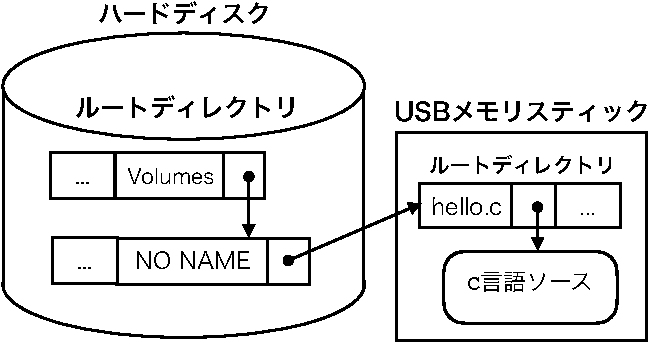
\includegraphics[scale=0.6]{Fig/mountTree-crop.pdf}
        \subcaption{マウント方式}
        \label{fig:mountTree}
      \end{center}
    \end{minipage}
    \begin{minipage}{0.49\columnwidth}
      \begin{center}
        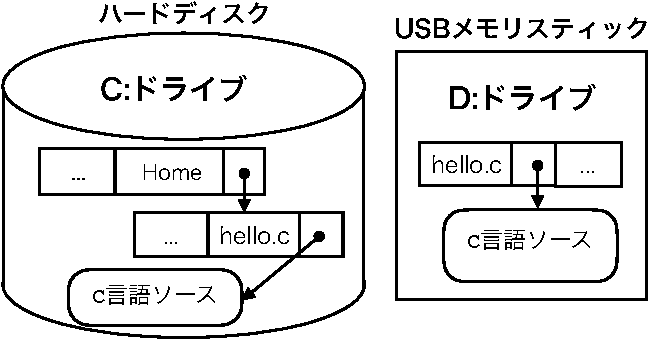
\includegraphics[scale=0.6]{Fig/mountDrive-crop.pdf}
        \subcaption{ドライブレター方式}
        \label{fig:mountDrive}
      \end{center}
    \end{minipage}
\end{myfig}

\begin{itemize}
\item[(a)] \emph{マウント方式} \\
  UNIXやmacOSでは新しいボリュームに格納されたファイルシステムを,
  既存のディレクトリに接続する(マウントする)方式が使用される.
  例えばmacOSにUSBメモリを接続した場合,
  自動的に\|/Volumes/VolName|\footnote{
    \texttt{VolName}はUSBメモリを初期化した時に決めたボリューム名である.
    購入時点で既に\texttt{NO NAME}や
    \texttt{UNTITLED}の名前を付けて初期化されていることが多い.
  }の位置にUSBメモリの内容が見えるようにマウントされる.
  新しいボリュームが追加されても,単一の木に全てが格納される.
  \figref{mountTree}の例では「C言語のソース」ファイルは,
  \|/Volumes/NO NAME/hello.c|のパスで参照できる.
\item[(b)] \emph{ドライブレター方式} \\
  Windowsではボリューム毎に新しい木を作りドライブレターで木を区別する.
  \figref{mountDrive}の例では,
  オペレーティングシステムがインストールされたドライブをCドライブ,
  USBメモリをDドライブのように決め,
  Cドライブのファイルは\|C:\Home\hello.c|のようなパス\footnote{
    Windowsではパスの区切りに使用する記号が
    「\texttt{/}」ではなく「\texttt{\bs}」になる.\\
    (日本語版のWindowsでは「\texttt{\bs}」が「\texttt{¥}」になる.)
  }で,Dドライブのファイルは\|D:\hello.c|のようなパスで表現する.
\end{itemize}

%============================================================================
\section{ファイルの属性}
\label{fileAttribute}
ファイルが持つ属性の例を以下に示す.
どのファイルシステムでも同じ属性を持っているとは限らない.
ここで示すのは一般的な例である.

\begin{itemize}
\item \emph{名前}:
  \figref{dirTree}ではファイルを格納するディレクトリが
  ファイル名を記録していたが,
  ファイル名もファイル属性の一つと考え,ファイル本体に記録する場合もある.
  また,FATファイルシステム(第\ref{fatFs}章参照)のように,
  全ての属性(ファイル名も含む)をディレクトリに記録する場合もある.
\item \emph{識別子}:
  ファイルシステム中でファイルを一意に識別できる番号などのこと.
\item \emph{型(タイプ)}:
  OSのカーネルがサポートしているファイルの種類のこと.
  UNIXでは,通常ファイル,ディレクトリファイル,シンボリックリンク,
  文字デバイス,ブロックデバイス等のファイル型が定義されている.
\item \emph{保護}:
  \|rwxrwxrwx|等のアクセス制御情報のことである.(次の節で詳しく説明する.)
\item \emph{日時}:
  作成日時,最終変更日時などのこと.
\item \emph{所有者}:
  所有者やグループ等を識別する情報のこと.
\item \emph{位置}:
  ディスク上でデータが記録されている場所を表す情報のこと.
\item \emph{サイズ}:
  ファイルが格納するデータの大きさをバイト単位で表す.
\item \emph{拡張}:
  そのファイルを開く時に使用するアプリケーションの名前や,
  セキュリティに関する追加属性のような情報のこと.
  OSカーネルが使い方を定めておらず,
  アプリケーション等が名前を付けて書き込める小さめのデータである.
  リスト\ref{extendedAttr}にmacOSの例を示す.

  \lstinputlisting[numbers=left,float=btp,
    caption=拡張属性の例,label=extendedAttr]{Lst/extendedAttr.txt}

  1行の\|ls -l@|コマンドは拡張属性の一覧も表示する.
  4行から「\|b.txtのエイリアス|」ファイルに\|com.apple.FinderInfo|という
  名前の32バイトの拡張属性ががあることが分かる.
  5行の\|xattr|コマンドで拡張属性の内容を表示してみた.
\end{itemize}

%============================================================================
\section{アクセス制御}
ファイルの保護属性に基づいたアクセス制御ができる.
UNIXでは\|rwxrwxrwx|の9ビットでファイルの「所有者」,「グループ」,
「その他のユーザ」の三者がRead/Write/eXecuteのどれをして良いか表現する.

より一般的な方式として\emph{ACL(Access Control List)}がある.
ファイル毎にどのユーザ(またはグループ)が何(\|rwx|より詳細)を
できるか(できないか)記録した順番付けされたリストをACLと呼ぶ.
リスト\ref{acl}にmacOSの例を示す.

\lstinputlisting[numbers=left,caption=macOSでACLを操作した例,
  float=btp,label=acl]{Lst/acl.txt}

3,4行の\|chmod|コマンドでファイル\|a.txt|にACLを追加している.
ACLの設定状況は\|ls -le|コマンドで確認できる.
ACLを持つファイルでは\|rwx|の右に\|+|が表示され,
次の行からACLの内容がリストされる.
ACLはリストの最初から順に,
許可・不許可が決まるまで評価される.

%ACLは詳細な制御を可能にするが可変長リストなので扱い難い.
最近のUNIX系オペレーティングシステム(macOS含む)では
ACLと\|rwx|方式を組合せて使用することができる.
その場合は,まず細かな制御が可能なACLを用いてチェックを行う.
ACLでアクセスを許可するかどうか決まらない場合に\|rwx|を用いる.

%============================================================================
\section{ファイルの種類}
ファイルの\emph{型属性}(\ref{fileAttribute}参照)は,
ファイルシステム(OSカーネル)が定めるファイルの種類を表現する.
「通常ファイル」,「ディレクトリ」,「シンボリックリンク」等の種類がある.
型が「通常ファイル」のファイルにはデータを格納することができる.
OSカーネルは通常ファイルのデータがバイトストリームであることは定めているが,
バイトストリームの中身には関与しない\footnote{実行形式プログラムは例外である}.

ファイル名の一部でファイルの種類を表現することが,
多くのオペレーティングシステムで慣例になっている.
ファイル名の最後が\|.xxx|のような文字列で終わっているのを
誰でも見たことがあると思う.
これを\emph{拡張子}と呼び,
ファイルに格納されたデータの種類を表現するために使用する.
多くのOSで拡張子は単にファイル名の一部である
\footnote{FATファイルシステムでは拡張子が特別扱いされている.}.
\tabref{filenameExtensions}によく使う拡張子と意味をまとめる
\footnote{表中\texttt{.app}拡張子だけはmacOSでディレクトリ名に付加される.}
\footnote{表の最初の3行(\texttt{.c}から\texttt{.xml})と
  \texttt{.ps},\texttt{.eps}はテキストファイルの一種である.}.

\begin{mytable}{btp}{よく見かけるファイルの拡張子}{filenameExtensions}
  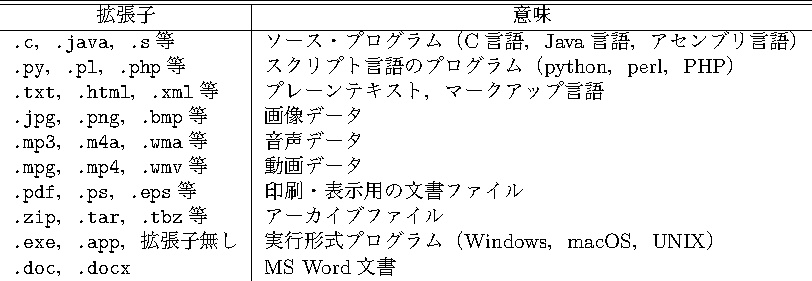
\includegraphics[scale=1.0]{Tbl/filenameExtensions.pdf}
\end{mytable}

%============================================================================
\section{ファイルシステムの操作}
ユーザがファイルを作ったり,
ファイルのデータを読み書きするために必要な操作を紹介する.

\subsection{ディレクトリ操作}
ユーザがファイルやディレクトリを自由に作ったり削除したりするために,
\tabref{dirOperations}に示すディレクトリ操作ができることが求められる.
表の右半分はUNIXで使用可能なAPIの例を示している.

\begin{mytable}{btp}{求められるディレクトリ操作}{dirOperations}
  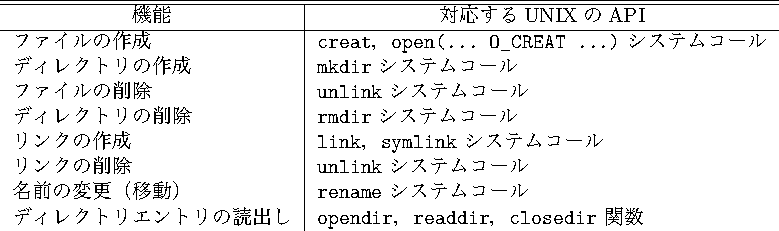
\includegraphics[scale=1.0]{Tbl/dirOperations.pdf}
\end{mytable}

\subsection{ファイルアクセス}
ユーザがファイルの内容や属性を読み書きするために
\tabref{fileOperations}の操作ができることが望ましい.

%\begin{enumerate}
\begin{description}
  %\item \emph{オープン}\\
\item[オープン]
  openシステムコールは,
  ファイルのパスとファイルに行う操作(読む・書く)等を引数に発行される.
  ファイルの保護属性と照らし合わせ,
  要求された操作が可能な場合のみファイルをオープンする.
  %\item \emph{読み書き}\\
\item[読み書き]
  ファイルをオープンした後,
  read/writeシステムコールを使用してファイルを先頭から
  最後に向けて\emph{シーケンシャルアクセス}することができる.
  読み書き位置を自由に変更できるlseekシステムコールを組合せることで,
  read/writeシステムコールは\emph{ランダムアクセス}にも使用できる.
  %\item \emph{クローズ}\\
\item[クローズ]
  closeシステムコールを用いてファイルをクローズする.
  ファイルがオープンされている間は,
  ファイル本体のリンクカウントが1増加したのと同じ状態になる.
  ファイルを削除しディレクトリからファイルが見えなくなっても
  ファイルの本体は削除されない.
  ファイルを消してもディスクの空き領域が増えない場合は,
  どれかプロセスがファイルをオープンしている可能性がある.
  %\item \emph{切り詰め}\\
\item[切り詰め]
  truncateシステムコールや\|O_TRUNC|フラグ付きで実行したopenシステムコールは,
  ファイルの長さを短く切り詰める.
  %\item \emph{プログラムの実行}\\
\item[プログラムの実行]
  execveシステムコールはファイルに格納されているプログラムを実行する.
  ファイルのフォーマットはexecveシステムコールが
  理解できるものである必要がある\footnote{
    ファイルはUNIXの実行可能な機械語形式かインタープリタに渡すデータである.
    ファイルの先頭が\texttt{\#!path}で始まる場合は
    \texttt{path}で指定されたインタープリタを起動し,
    ファイルの内容を解釈・実行させる.
  }.
  %\item \emph{属性の読み書き}\\
\item[属性の読み書き]
  chmodシステムコール等でファイルの属性を書き換えることができる.
  また,statシステムコールはファイル属性の読み出しに使用できる.
  %\end{enumerate}
\end{description}

\begin{mytable}{btp}{求められるファイル操作}{fileOperations}
  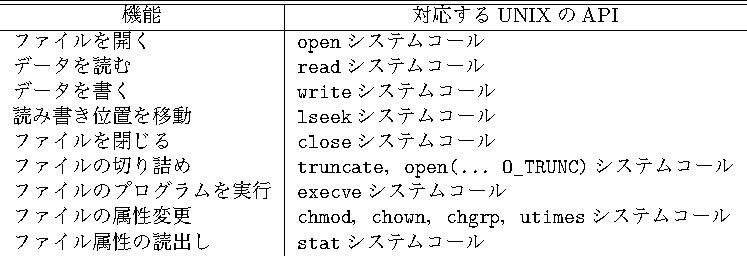
\includegraphics[scale=1.0]{Tbl/fileOperations.pdf}
\end{mytable}

\subsection{ファイルの共有とロック}
ファイルを複数のプロセスで安全に共有するためにロックのメカニズムが求められる.
「\ref{readersWritersProglem}リーダ・ライタ問題」でも紹介した
\emph{共有ロック(shared lock)}と
\emph{排他ロック(exclusive lock)}を
ファイルに掛けるUNIXの仕組みを紹介する.

UNIXではファイルをロックするためにflockシステムコールが準備されている.
flockは,引数に定数\|LOCK_SH|を渡すと共有ロックを,
定数\|LOCK_EX|を渡すと排他ロックをファイルに掛ける.
共有ロックは複数のプロセスが同時に掛けることができる.
排他ロックはファイルが全くロックされていない場合のみ掛けることができる.
排他ロックされている間は,
他のプロセスはどちらのロックも掛けることができなくなる.
ロックが掛けられない時,
flockシステムコールがブロックしないようにするには,
上記の定数に\|LOCK_NB|フラグを(ビット毎の論理和で)合わせてflockに渡す.
以下にmacOSのflockの書式を示す.

\newpage
\begin{lstlisting}[numbers=none]
  #include <sys/file.h>
  #define   LOCK_SH   1    // 共有ロック
  #define   LOCK_EX   2    // 排他ロック
  #define   LOCK_NB   4    // ブロックしない
  #define   LOCK_UN   8    // ロック解除
  int flock(int fd, int operation);
\end{lstlisting}

また,openシステムコールを使用してファイルにロックを掛けることもできる.
openシステムコールは,
引数に\|O_SHLOCK|フラグを指定すると共有ロックを,
引数に\|O_EXLOCK|フラグを指定すると排他ロックを,
ファイルのオープン時に自動的に掛ける.

\subsection{ワーキングディレクトリの変更}
ワーキングディレクトリ(カレントディレクトリ)はプロセス毎に決められるので,
プロセスの操作に分類するほうが正しいかもしれないがここで紹介しておく.
UNIXではchdirシステムコールを用いて
プロセスが自身をワーキングディレクトリを変更する.
初期のワーキングディレクトリは親プロセスから引き継がれる.
以下にchdirの書式を示す.

\begin{lstlisting}[numbers=none]
  #include <unistd.h>
  int chdir(const char *path);
\end{lstlisting}

%============================================================================
\section{ファイルシステムの健全性}
停電,OSのクラッシュ,ハードウェアの故障等により,
ファイルシステムが壊れてしまうことがある.
ファイルシステムの一貫性をチェックし必要に応じて修復する方法と,
壊れ難いファイルシステムについて紹介する.

\subsection{一貫性チェック}
\label{unmountFlag}
コンピュータが異常停止をしてしまった場合,
次回の起動時にファイルシステムの一貫性をチェックする.
例えばUNIXでは,正常なシステム終了時にはファイルシステムに
「正常にファイルシステムがアンマウントされた」印が残る.
次回のシステム起動時に,印が付いていないファイルシステムについて
fsck\footnote{
  UNIXのfsckにあたるコマンドは,
  Windows では chkdsk や scandisk,macOS では Disk First Aid 等である.
}コマンドが自動的に実行される.

fsckコマンドは,使用中の\inode やディレクトリの内容等を突き合わせ
矛盾がないか確認する.
例えば,使用中の\inode がどのディレクトリからも参照されていない
(リンクカウントが間違っている),
同じデータブロックが複数の\inode から参照されている等の矛盾が予想される.
fsckコマンドは,チェック結果からファイルシステムの修復を行う.

この方式は\emph{メタデータ}\footnote{
  ファイルシステムの構造を管理するデータのこと.
  FATファイルシステムのディレクトリやFAT,
  UNIXの\inode やディレクトリエントリ等が該当する.}
の矛盾を解消するが元通りにする分けではない.
メタデータに矛盾があったファイルやディレクトリが失われたり,
更新したはずのファイルが更新途中の状態になったりする可能性がある.
また,fsckが終了するまで\footnote{
  一貫性のチェックには数分かかる場合も多い.その間,システムが使用できない.}
システムが起動しない.

\subsection{ジャーナリング・ファイルシステム}
データベースで使用されたWAL(Write Ahead Logging)を
ファイルシステムに応用したものである.
NTFS\footnote{Windows のファイルシステムである.},
ext3,ext4\footnote{Linux のファイルシステムである.},
HFS+\footnote{macOS のファイルシステムである.}等は
ジャーナリングファイルシステムである.

システムがクラッシュした後でも,
ジャーナリングファイルシステムの状態は,
システムコールが完了した後かシステムコールを実行し始める前か,
どちらかに落ち着く.
システムコールを実行する途中の中途半端な状態になりファルシステムが
壊れることはない.
\figref{journaling}にジャーナリングファイルシステムの仕組みを,
以下におおよその動作原理を示す.

\begin{myfig}{btp}{ジャーナリングファイルシステムの仕組み}{journaling}
  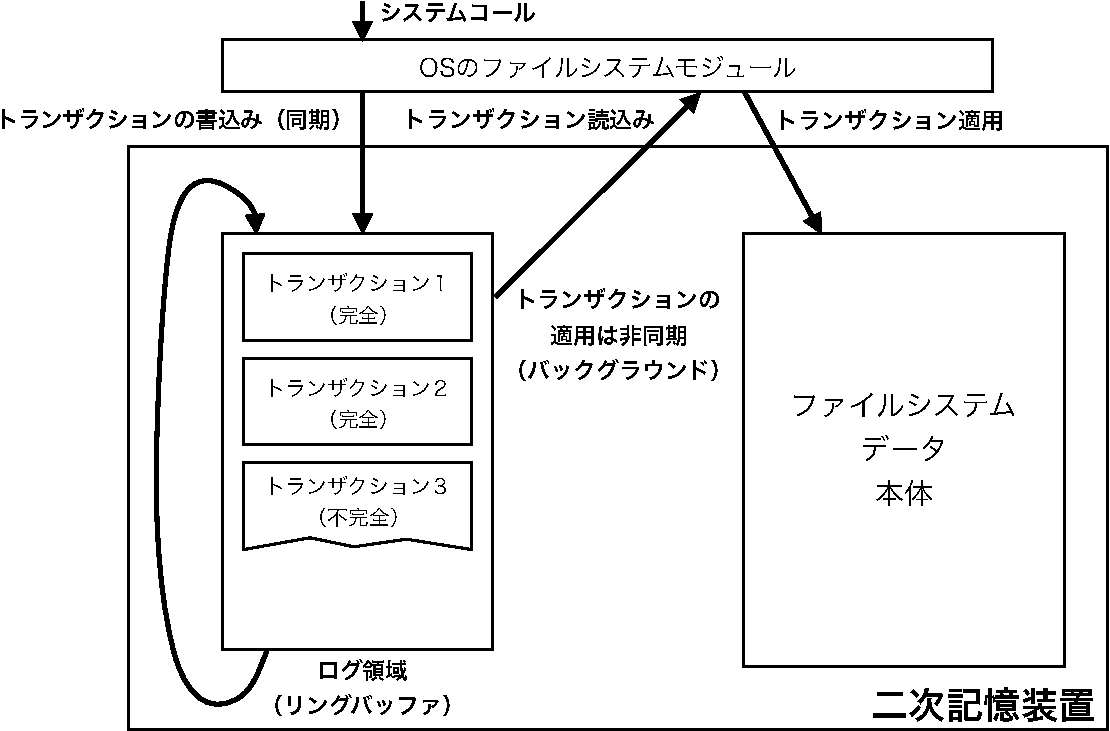
\includegraphics[scale=.75]{Fig/journaling-crop.pdf}
\end{myfig}

\begin{enumerate}
\item システムコールによる一連の操作はトランザクションとして
  ログ領域\footnote{同一ディスクの別領域の場合と別ディスクの場合がある.
  }に記録する.
\item トランザクションの書込み完了でシステムコールは完了し,
  ユーザプロセスは次の処理を開始できる.
\item OSはバックグラウンド処理でログ領域からトランザクションを順に取り出し,
  ファイルシステム本体に適用する.
\item システムがクラッシュした場合,
  ログ領域への書込みが完了していたトランザクションは
  再実行しファイルシステム本体に完全に反映する.
  書込み途中だったトランザクションは無視する.
\end{enumerate}

トランザクションはログ領域にシーケンシャルに書き込まれる.
ファイルシステム本体の操作はランダムアクセスが必要なので時間がかかるが,
シーケンシャルアクセスだけで完了するトランザクション書込みは短時間に終わる.
システムコールを短時間に終わらせることができる.

なお,ログ領域を通して操作するのはメタデータだけのシステムが多い.
ファイルシステムの構造が不整合を起こすことは予防できるが,
ファイル内のデータを守ることはできない.

%============================================================================
\section{まとめ}
この章ではファイルシステムが備えるべき機能や概念に付いて学んだ.
ファイルシステムは,二次記憶装置を抽象化・仮想化したファイルを
ユーザに提供するオペレーティングシステムの仕組みである.
本章の多くの部分でUNIX(またはmacOS)を例にしたが,
基本はWindows等でも共通である.

現代のオペレーティングシステムは,
ファイルを木構造のディレクトリシステムに格納する方式を採用している.
ディレクトリシステムから一つのファイルを選択するために\emph{パス}を用いる.
パスには\emph{ルートディレクトリ}を起点とする\emph{絶対パス}と,
\emph{ワーキングディレクトリ}を起点とする\emph{相対パス}がある.

ファイルに別名を付ける方法として,
\emph{ハードリンク},\emph{シンボリック}が知られている.
これらはファイルシステムの仕組みとして実装され,
オペレーティングシステムのカーネル内で処理される.
これらの他に,ファイルシステムの外で実装される別名の仕組みもある.
WindowsのショートカットやmacOSのエイリアスがそれに該当する.

複数のボリュームがある時,
二つ目以降のボリュームを既存のディレクトリに
接続(マウント)する方式を\emph{マウント方式}と呼ぶ.
一方で,ボリューム毎にボリュームを表す文字を決めて区別する方式を
\emph{ドライブレター方式}と呼ぶ.

ファイルは,保護,最終変更時刻,所有者等の属性を持つ.
本章では代表的な属性を紹介した.
また,ファイルは保護属性に基づいたアクセス制御ができることが望ましい.
ファイルはファイルシステムが定めた型(タイプ)を表す属性を持っている.
この属性により,通常ファイル,ディレクトリ,シンボリックリンク等を区別する.
ファイルが,どのアプリケーションのデータを格納しているかは,
ファイル名の一部(拡張子)で区別する.

ファイルシステムは,ファイルの読み・書き,ファイルの作成・削除などの
いくつかの基本的な機能を備える必要がある.
また,これらの機能をユーザプログラムが呼び出して使用できるように
システムコールを提供する必要がある.
本章では代表的な操作(システムコール)を紹介した.

%============================================================================
\section*{練習問題}
\begin{enumerate}
  \renewcommand{\labelenumi}{\ttfamily\arabic{chapter}.\arabic{enumi}}
  \setlength{\leftskip}{1em}
\item 次の言葉の意味を説明しなさい.
  \begin{enumerate}
  \item ディレクトリシステム
  \item パス,絶対パス,相対パス
  \item ディレクトリ,ファイル
  \item ハードリンク,シンボリックリンク
  \item ショートカット,エイリアス
  \item マウント,ドライブレター
  \item 拡張属性,ACL
  \item 拡張子
  \item 共有ロック・排他ロック
  \item 一貫性チェック
  \item ジャーナリング・ファイルシステム
  \end{enumerate}
\item 自分が使用しているオペレーティングシステムについて調査しなさい.\\
  (GUIではなく,CLIのコマンドを用いるとより詳しい観察ができる場合がある.)
  \begin{enumerate}
  \item ショートカット(Windows),エイリアス(macOS)
  \item ファイルの属性(保護,日時,所有者,サイズ等)
  \item 拡張属性が使用できるオペレーティングシステムか?
  \item ACLが使用できるオペレーティングシステムか?
  \item USBメモリにはどのようなパスで到達できるか?
  \item ファイルシステムの一貫性をチェックするコマンドは何か?
  \end{enumerate}
\item 自分が使用しているオペレーティングシステムで試してみなさい.
  \begin{enumerate}
  \item ショートカット(Windows)やエイリアス(macOS)を作成し,
    予定通りに働くかGUIとCLIの両方で試してみなさい.
\begin{lstlisting}
  # macOSの場合の実行例
  $ echo aaa > a.txt
  $ open a.txt
  $ open a.txtのエイリアス      <--- エイリアスはGUIで作る
  $ cat a.txt
  $ cat a.txtのエイリアス
\end{lstlisting} %$
  \item UNIXやmacOSで実行して結果が異なる理由を考察しなさい.
\begin{lstlisting}
  # ハードリンクの場合          # シンボリックリンクの場合
  $ echo aaa > a.txt          $ echo aaa > a.txt
  $ echo bbb > b.txt          $ echo bbb > b.txt
  $ ln a.txt c.txt            $ ln -s a.txt c.txt
  $ mv a.txt d.txt            $ mv a.txt d.txt
  $ mv b.txt a.txt            $ mv b.txt a.txt
  $ cat c.txt                 $ cat c.txt
\end{lstlisting} %$
  \item ショートカットやエイリアスの振る舞いを調べる.\\
    (リンク先ファイルを削除・移動・別ファイルに置換えた場合など)
  \item ACLの追加・削除とその効果を確認する.
  \end{enumerate}
\end{enumerate}
